\chapter{Měření intenzity větrání pomocí techniky indikačních plynů}\label{navesti:prutoky}
Hlavním zdrojem této kapitoly je~\cite{metodika}.

Technika indikačních plynů dovoluje určit objemové průtoky vzduchu mezi specifikovanými kompartmenty zkoumaného objektu, jakož i průtoky vzduchu ze všech zón do vnějšího prostředí (exfiltrace) a průtoky z vnějšího prostředí do všech zón (infiltrace). Z exfiltrací a objemů všech zón lze určit výměnu vzduchu objektu. Jedná se o pasivní techniku, a tudíž poskytuje pouze průměrné hodnoty za celou dobu měření. Proměřování objektu pomocí této techniky pro zjednodušení nazýváme měření ventilace objektu.

Technika byla vyvinuta Státním ústavem radiační ochrany, v. v. i. (SÚRO) a její správnost byla ověřena s obdobnými technikami používanými v zahraničí. Vše o ní je popsáno v certifikované metodice (\cite{metodika}), podle níž se postupovalo i při měřeních provedených v rámci této práce. Principem techniky je detekce vhodně použitých indikačních plynů, jejichž zdroje jsou rozmístěny po objektu a které mají definovaný konstantní přísun do zón. Ze známosti těchto přísunů do jednotlivých zón, z odezev detektorů a z dalších faktů je možné určit hledané veličiny, tj. objemové průtoky vzduchu a výměnu vzduchu objektu.

Při měření se používají tzv. vyvíječe, ze kterých se odpařují indikační plyny, dále TD detektory, na které se indikační plyny sorbují. Pomocnými zařízeními jsou především kontinuální měřidla teploty testo 174H a laserové dálkoměry pro určení objemů kompartmentů. Při vyhodnocování se používá plynový chromatograf s termální desorpcí. Vše je podrobněji popsáno v dalším oddíle.
\section{Přístroje a pomůcky}
Dva vyvíječe a dva TD detektory jsou k vidění v obr.~\ref{fig:prutoky_vyvijece_detektory}.
\begin{figure}[ht]
    \centering
    \begin{subfigure}[b]{0.4\textwidth}
        \centering
        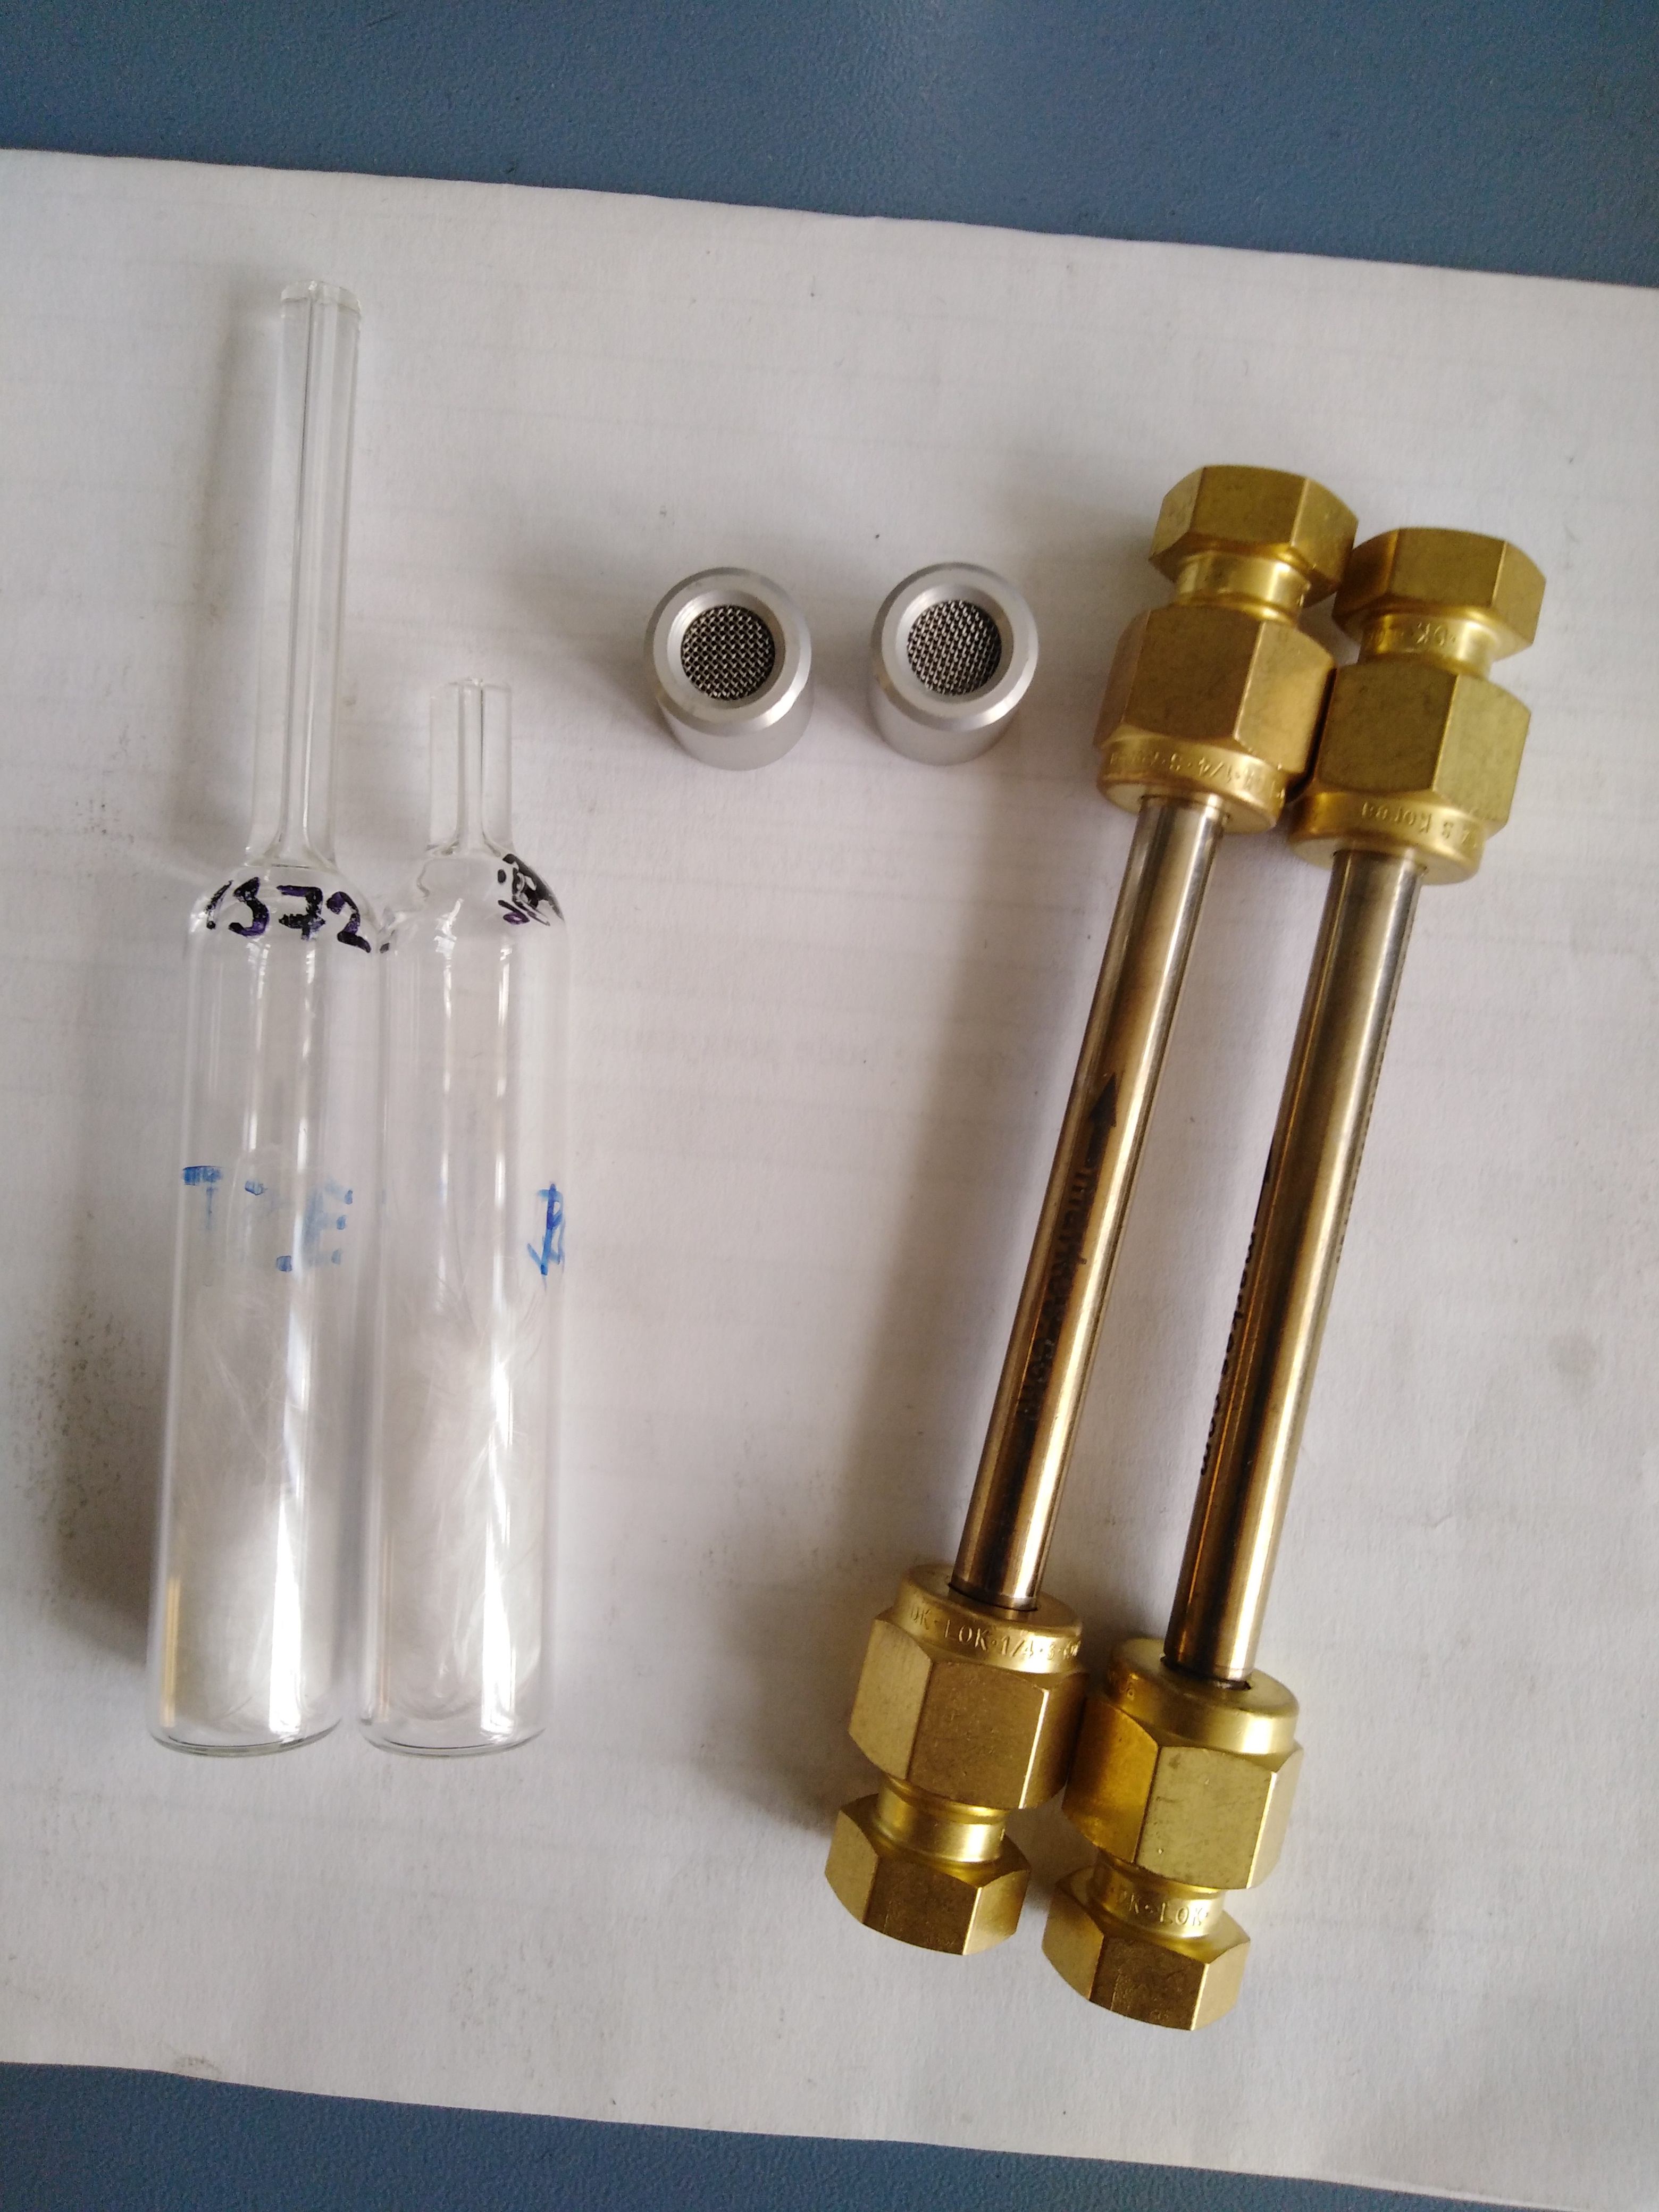
\includegraphics[width=.95\textwidth]{vyvijece_detektory.jpg}
        \caption{}
        \label{fig:prutoky_vyvijece_detektory}
    \end{subfigure}
    \begin{subfigure}[b]{0.35\textwidth}
        \centering
        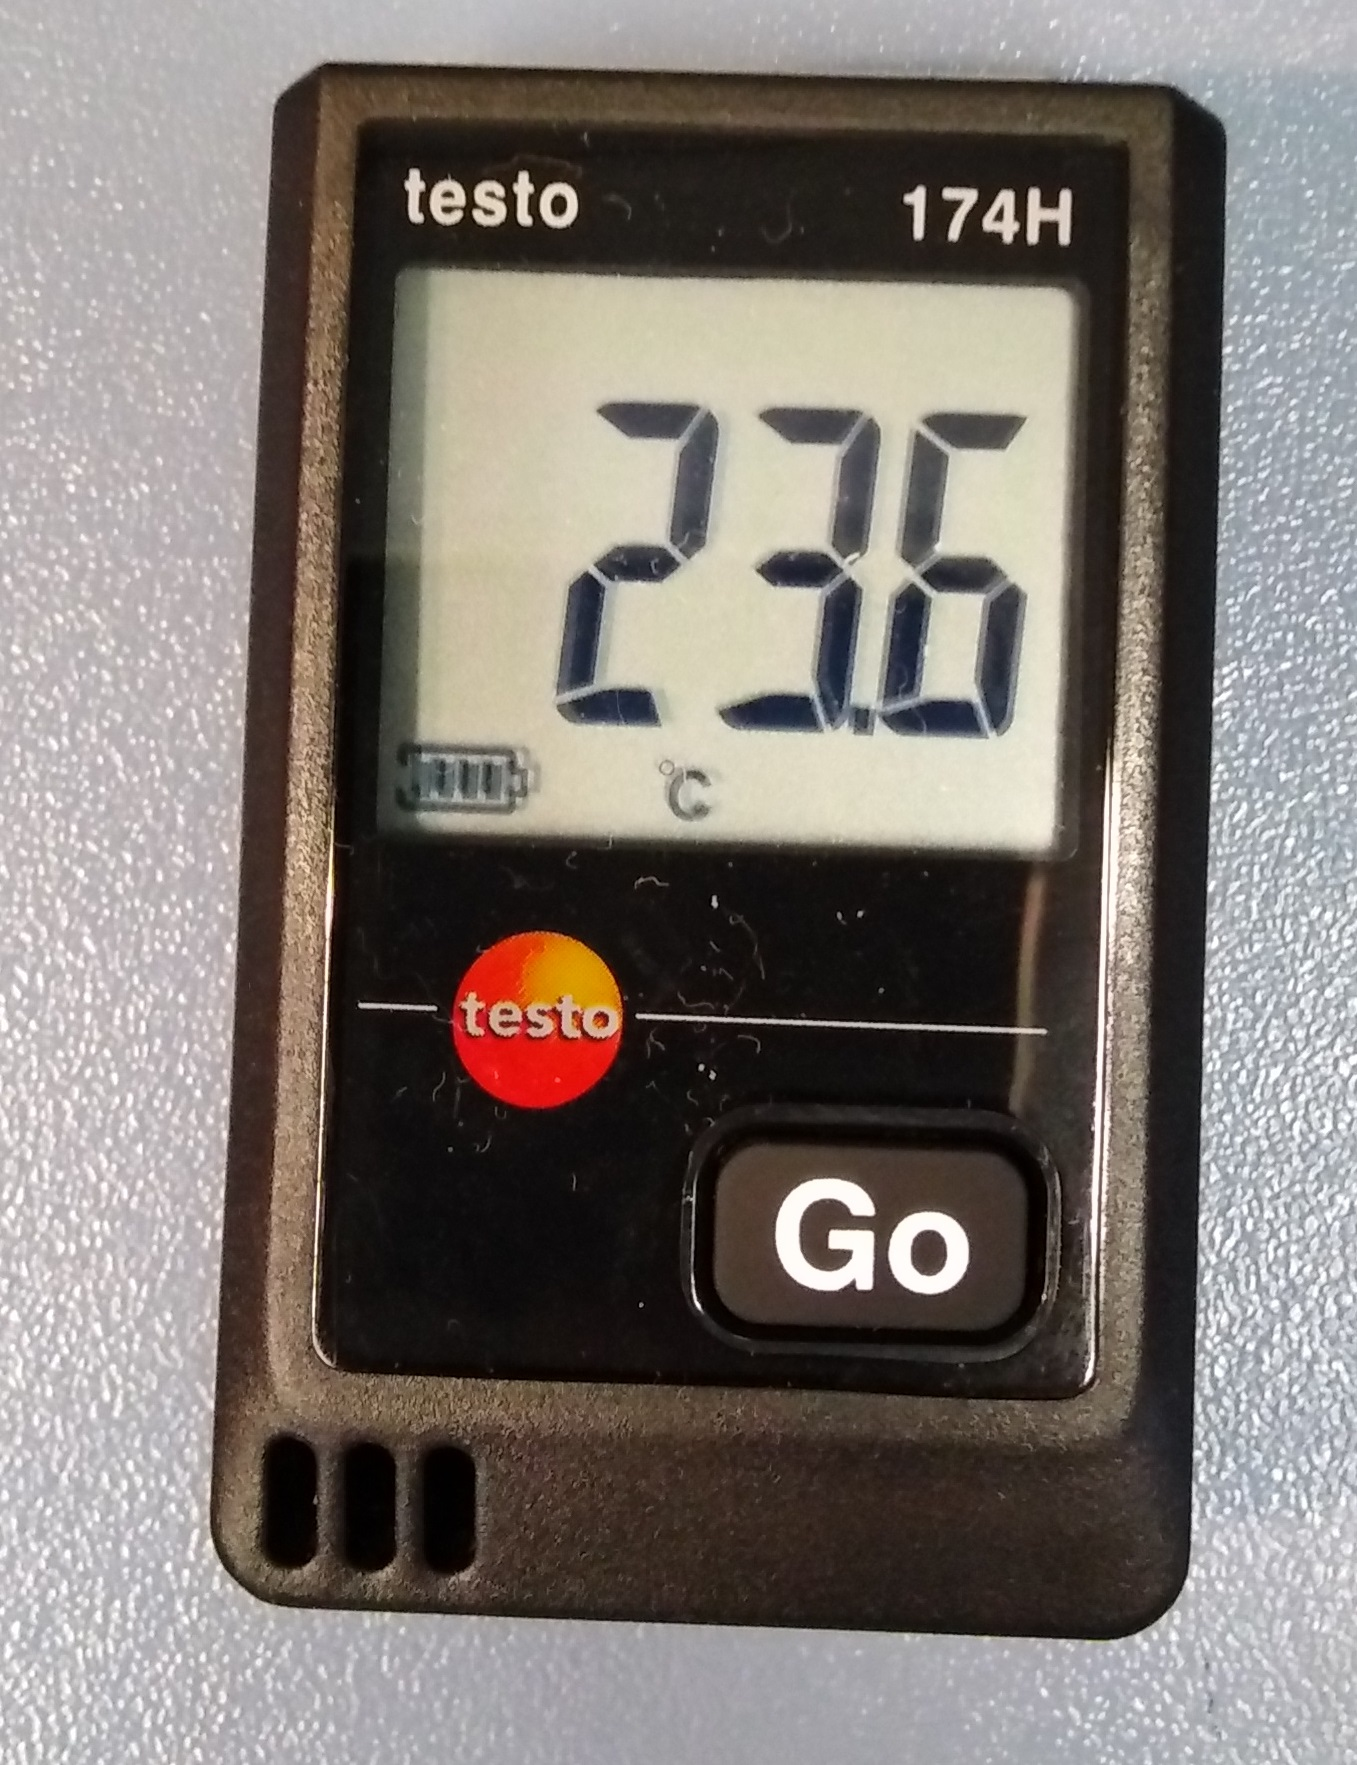
\includegraphics[width=.85\textwidth]{testo.jpg}
        \caption{}
        \label{fig:prutoky_testo}
    \end{subfigure}
    \caption{V (a) jsou zobrazeny vyvíječe (skleněné trubičky) a TD detektory (kovové zlatě zabarvené trubice). Mezi vyvíječi a TD detektory jsou difúzní uzávěry. V (b) je digitální měřič teploty testo 174H.}
\end{figure}
\begin{description}
    \item[Vyvíječ] je kapilára vhodné tloušťky, plynově neprodyšná, většinou ze skla, obsahující kapalnou fázi příslušného indikačního plynu s difúzní membránou, která řídí definované a konstantní odpařování (emise indikačního plynu). Emise je dále ovlivněna tloušťkou kapiláry a z vnějších faktorů by ji měla teoreticky ovlivňovat pouze okolní teplota. Při zjišťování, kolik plynu se odpařilo, se používají laboratorní váhy SARTORIUS. Teplota okolního prostředí při měření je zjištěna pomocí digitálního teploměru testo~174H (obr.~\ref{fig:prutoky_testo}).
    \item[TD detektor] je zařízení sloužící k záchytu indikačních plynů a tím k měření jejich koncentrace ve vzduchu. Je plněn vhodným sorbentem vzhledem k použitým indikačním plynům. V SÚRO se používají sorbenty Chromosorb 102, TENAX-TA 35/60 a TENAX-TA 80/100~\cite{metodika}. Jejich výrobcem je firma MARKES~\cite{markes}. Jedná se o kovovou trubici opatřenou kovovými uzávěry, které by neměly propustit žádný s indikačních plynů dovnitř k sorbentu. Pro měření se jeden závěr (z konstrukce trubice je zřejmé který) odšroubuje a nahradí se difúzním uzávěrem (viz obr.~\ref{fig:prutoky_vyvijece_detektory}). Po skončení měření je difúzní uzávěr vyměněn opět za kovový.
    \item[Plynový chromatograf s termální desorpcí] slouží k určení množství indikačních plynů, které se zachytily v sorbentu v TD detektoru. Z TD detektoru jsou odstraněny oba dva kovové uzávěry a pak je umístěn na příslušné místo do chromatografu. Poté je promýván nosným plynem, kterým je hélium, na který se pomocí termální desorpce zachytávají indikační plyny nasorbované uvnitř TD detektoru. Nosný plyn s indikačními plyny je veden do separačních kapilárních kolon, kde dochází k oddělování jednotlivých indikačních plynů od sebe. Následně jsou již oddělené indikační plyny kvantitativně analyzovány v detektoru typu ECD nebo FID. Plynový chromatograf, který byl použit pro naše měření, je na obr.~\ref{fig:prutoky_chromatograf}.
    \item[Testo 174H] je digitální teploměr. Teplota je potřeba znát k přesnému určení emise vyvíječe a také pro výpočet hmotnostní koncentrace indikačního plynu z odezvy TD detektoru.
    \item[Laserový dálkoměr] pro určení objemů jednotlivých kompartmentů/zón.
    \item[Další pomůcky:] přesné laboratorní dávkovače kapalné fáze indikačních plynů do vyvíječů s rozlišením 5$\mu$l; přesné váhy SARTORIUS s přesností na desetinu miligramu pro měření a kontrolu emise indikačního plynu z vyvíječů; pinzety, nosný plyn do chromatografu a další spotřební materiál.
\end{description}


\begin{figure}[ht]
    \centering
    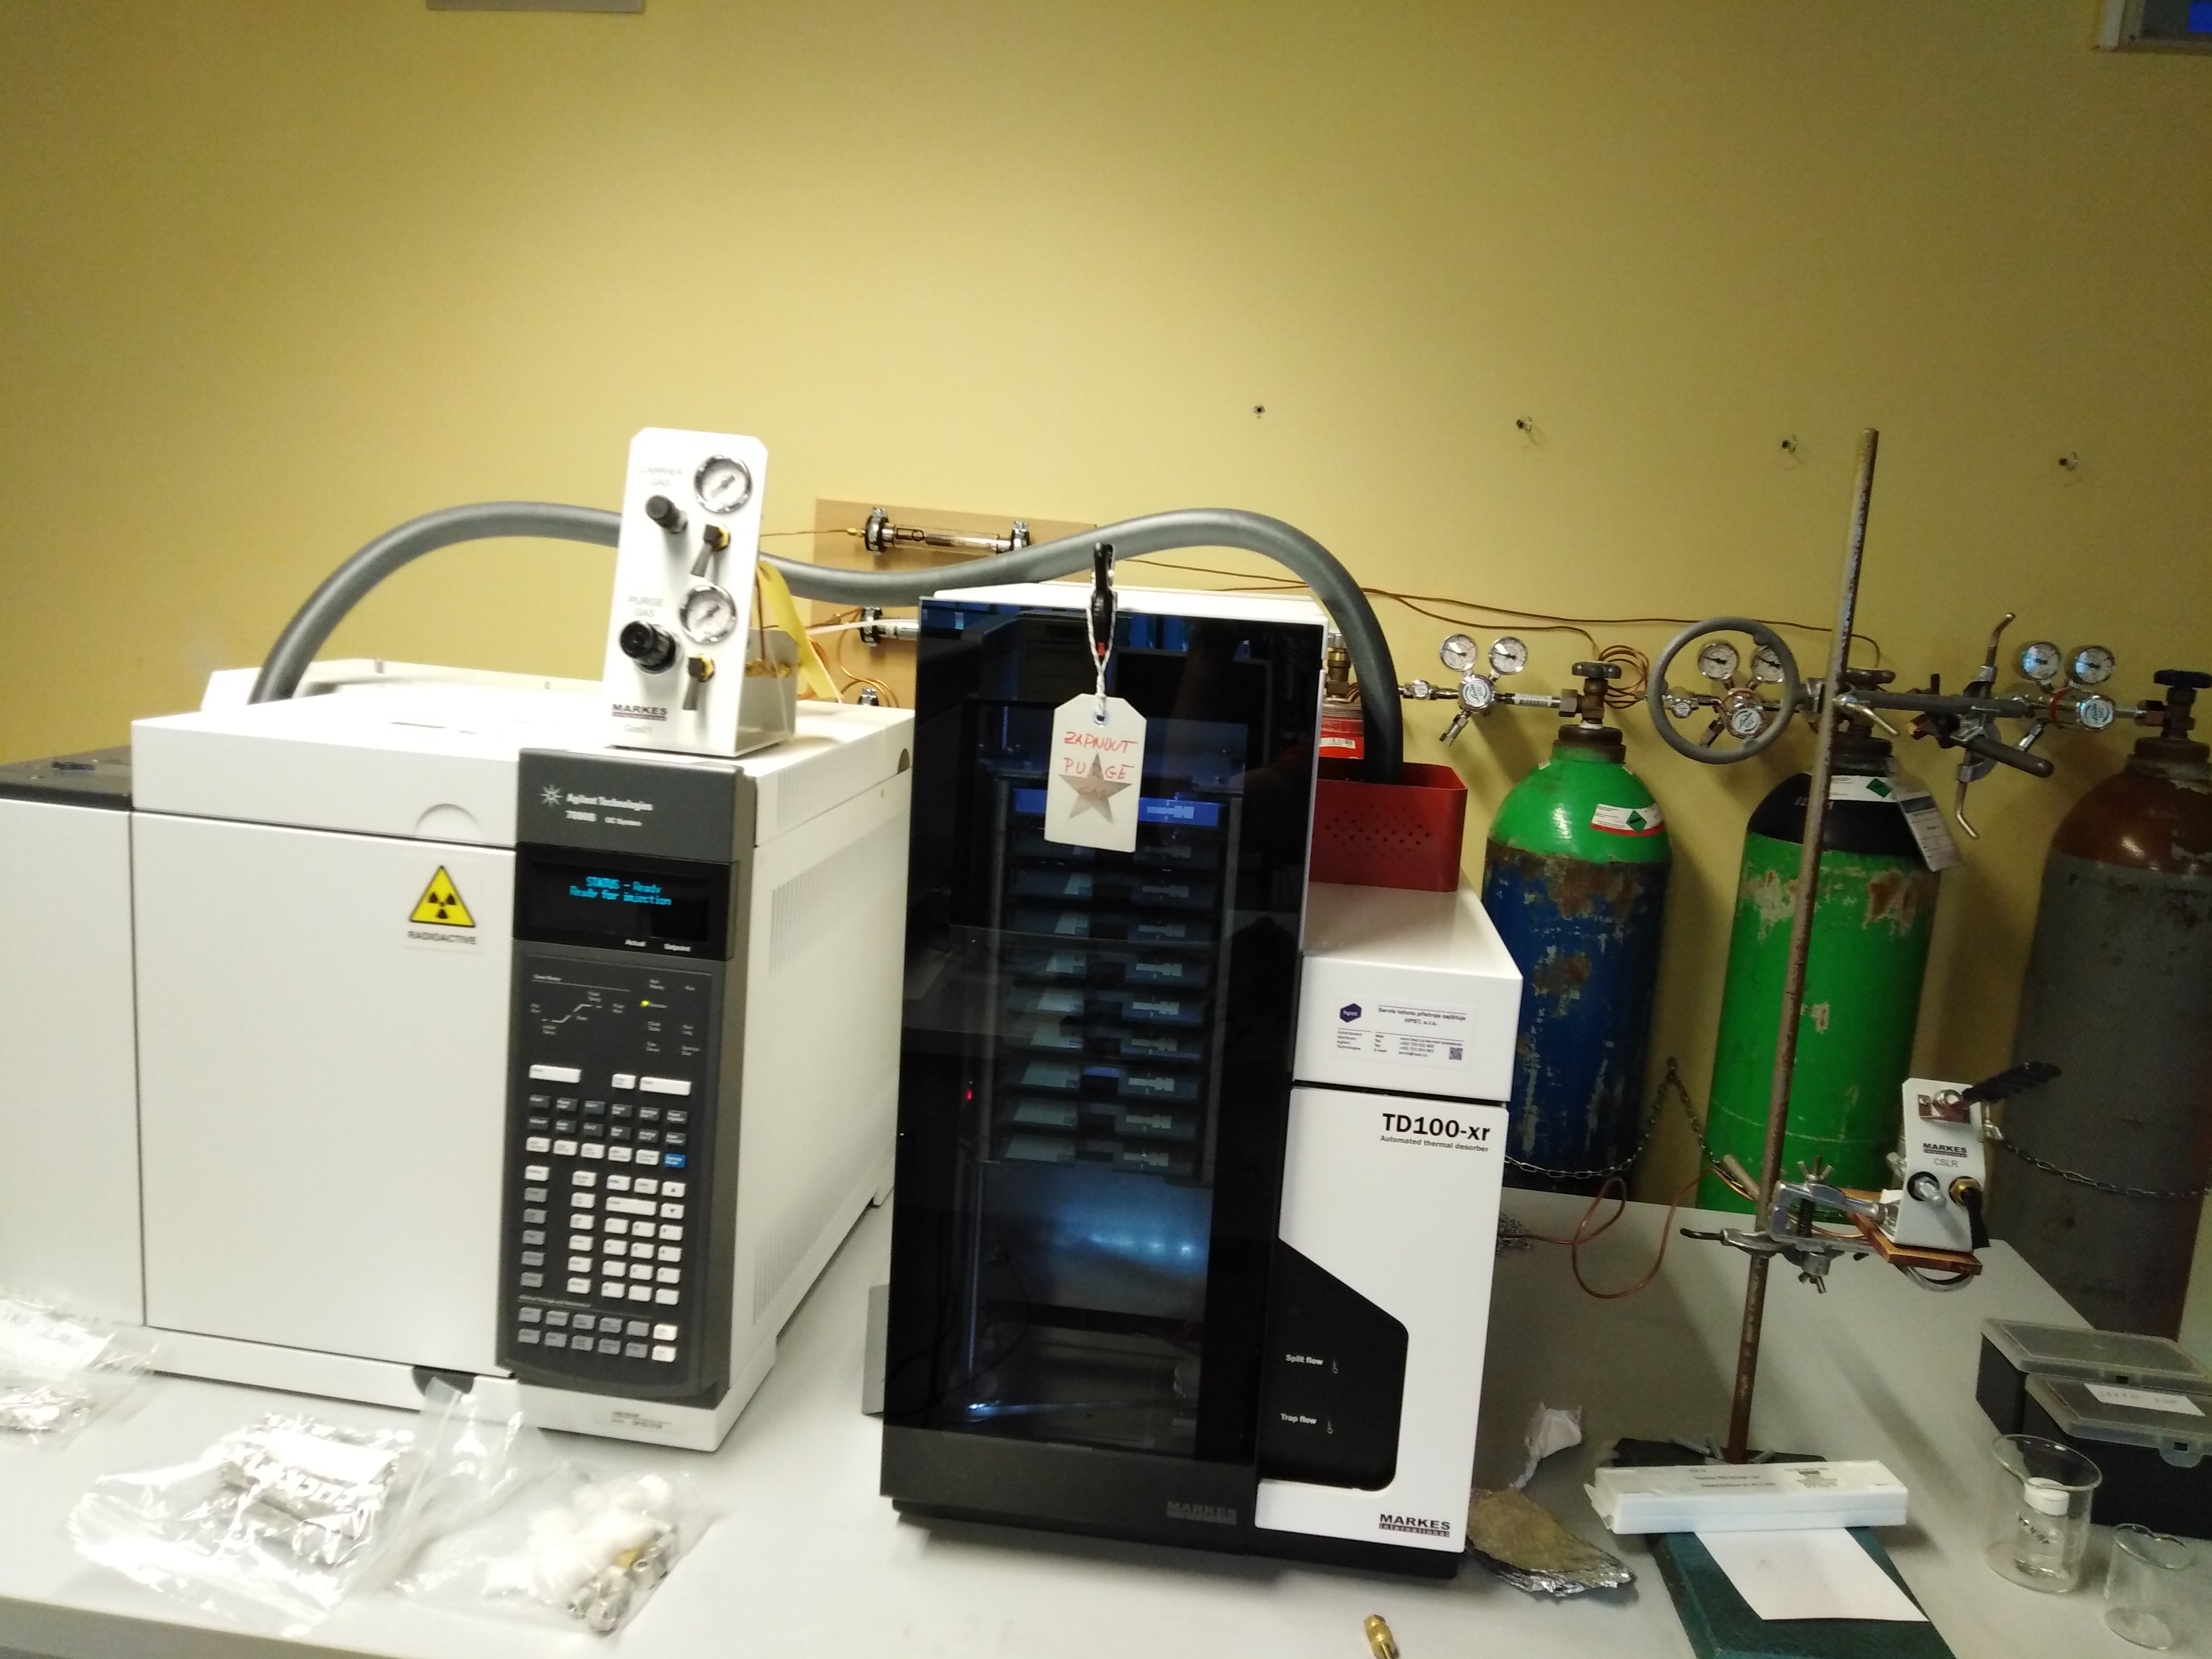
\includegraphics[width=.7\textwidth]{chromatograf_celkove.jpg}
    \caption{Plynový chromatograf Shimadzu GC 17A-FID/ECD s termální desorpcí, pomocí níž se indikační plyny desorbují z TD detektoru na nosný plyn (hélium). Úplně napravo je v popředí na stole vidět držák sloužící ke kalibraci chromatografu, za držákem v pozadí jsou vidět tlakové láhve s nosným plynem. V přístroji uprostřed obrázku jsou umístěny kapilární kolony, ve kterých probíhá separace jednotlivých indikačních plynů, a v přístroji úplně napravo dochází k jejich kvantitativnímu zpracování (pomocí detektoru ECD nebo FID). Více informací viz~\cite{metodika}.}
    \label{fig:prutoky_chromatograf}
\end{figure}

\section{Pracovní postup}
\subsection{Příprava měření}
Zkoumaný objekt s více patrami rozdělujeme na zóny většinou podle podlaží. Pokud se jedná o jednopodlažní objekt, pak vzhledem k zaměření tohoto výzkumného úkolu objekt rozdělíme tak, aby v každé zóně byla pokud možno homogenní koncentrace radonu. Platí, že máme-li $N$ kompartmentů, pak potřebujeme minimálně $N$ indikačních plynů (tracerů). 

Před měřením je potřeba připravit všechny potřebné vyvíječe, TD detektory, laserový dálkoměr a teploměry testa. To obnáší nastavit emisi vyvíječů tak, aby nedošlo k nasorbování většího množství indikačních plynů na TD detektory než jejich měřící rozsah. Při tom je zapotřebí vzít do úvahu velikost zón, větrací návyky obyvatel objektu a vnější teplotu v průběhu měření. Pokud dojde k nasorbování nějakého indikačního plynu přes měřící rozsah u některého z TD detektorů, pak je tento TD detektor sice stále možné vyhodnotit, ale s obrovskou nepřesností, která navíc nelze ani určit. 

U TD detektorů by mělo být překontrolováno dotažení kovových uzávěrů.
\subsection{Přeprava}
Uvažujeme přepravu autem. Při přepravě by neměly být vyvíječe a TD detektory umístěny u sebe, i když se uvádí, že skrz kovový uzávěr se do TD detektoru nemůže indikační plyn dostat. Ideální je, když jsou TD detektory umístěny na přední palubce u řidiče a vyvíječe v kufru. Pak totiž proudění vzduchu v autě zabraňuje indikačním plynům odpařujícím se z vyvíječů dostat se k TD detektorům. Pro jistotu by mely být TD detektory být zabaleny do igelitového pytlíku. Pro zaručení přesnosti jsou navíc používány dva tzv. trip blank TD detektory, což jsou TD detektory, které cestují s ostatními TD detektory, ale neosazují se do objektu a jsou nich neustále kovové uzávěry. Na obr.~\ref{fig:prutoky_vyvijecePreprava} jsou vidět vyvíječe připravené k přepravě.
\begin{figure}[ht]
    \centering
    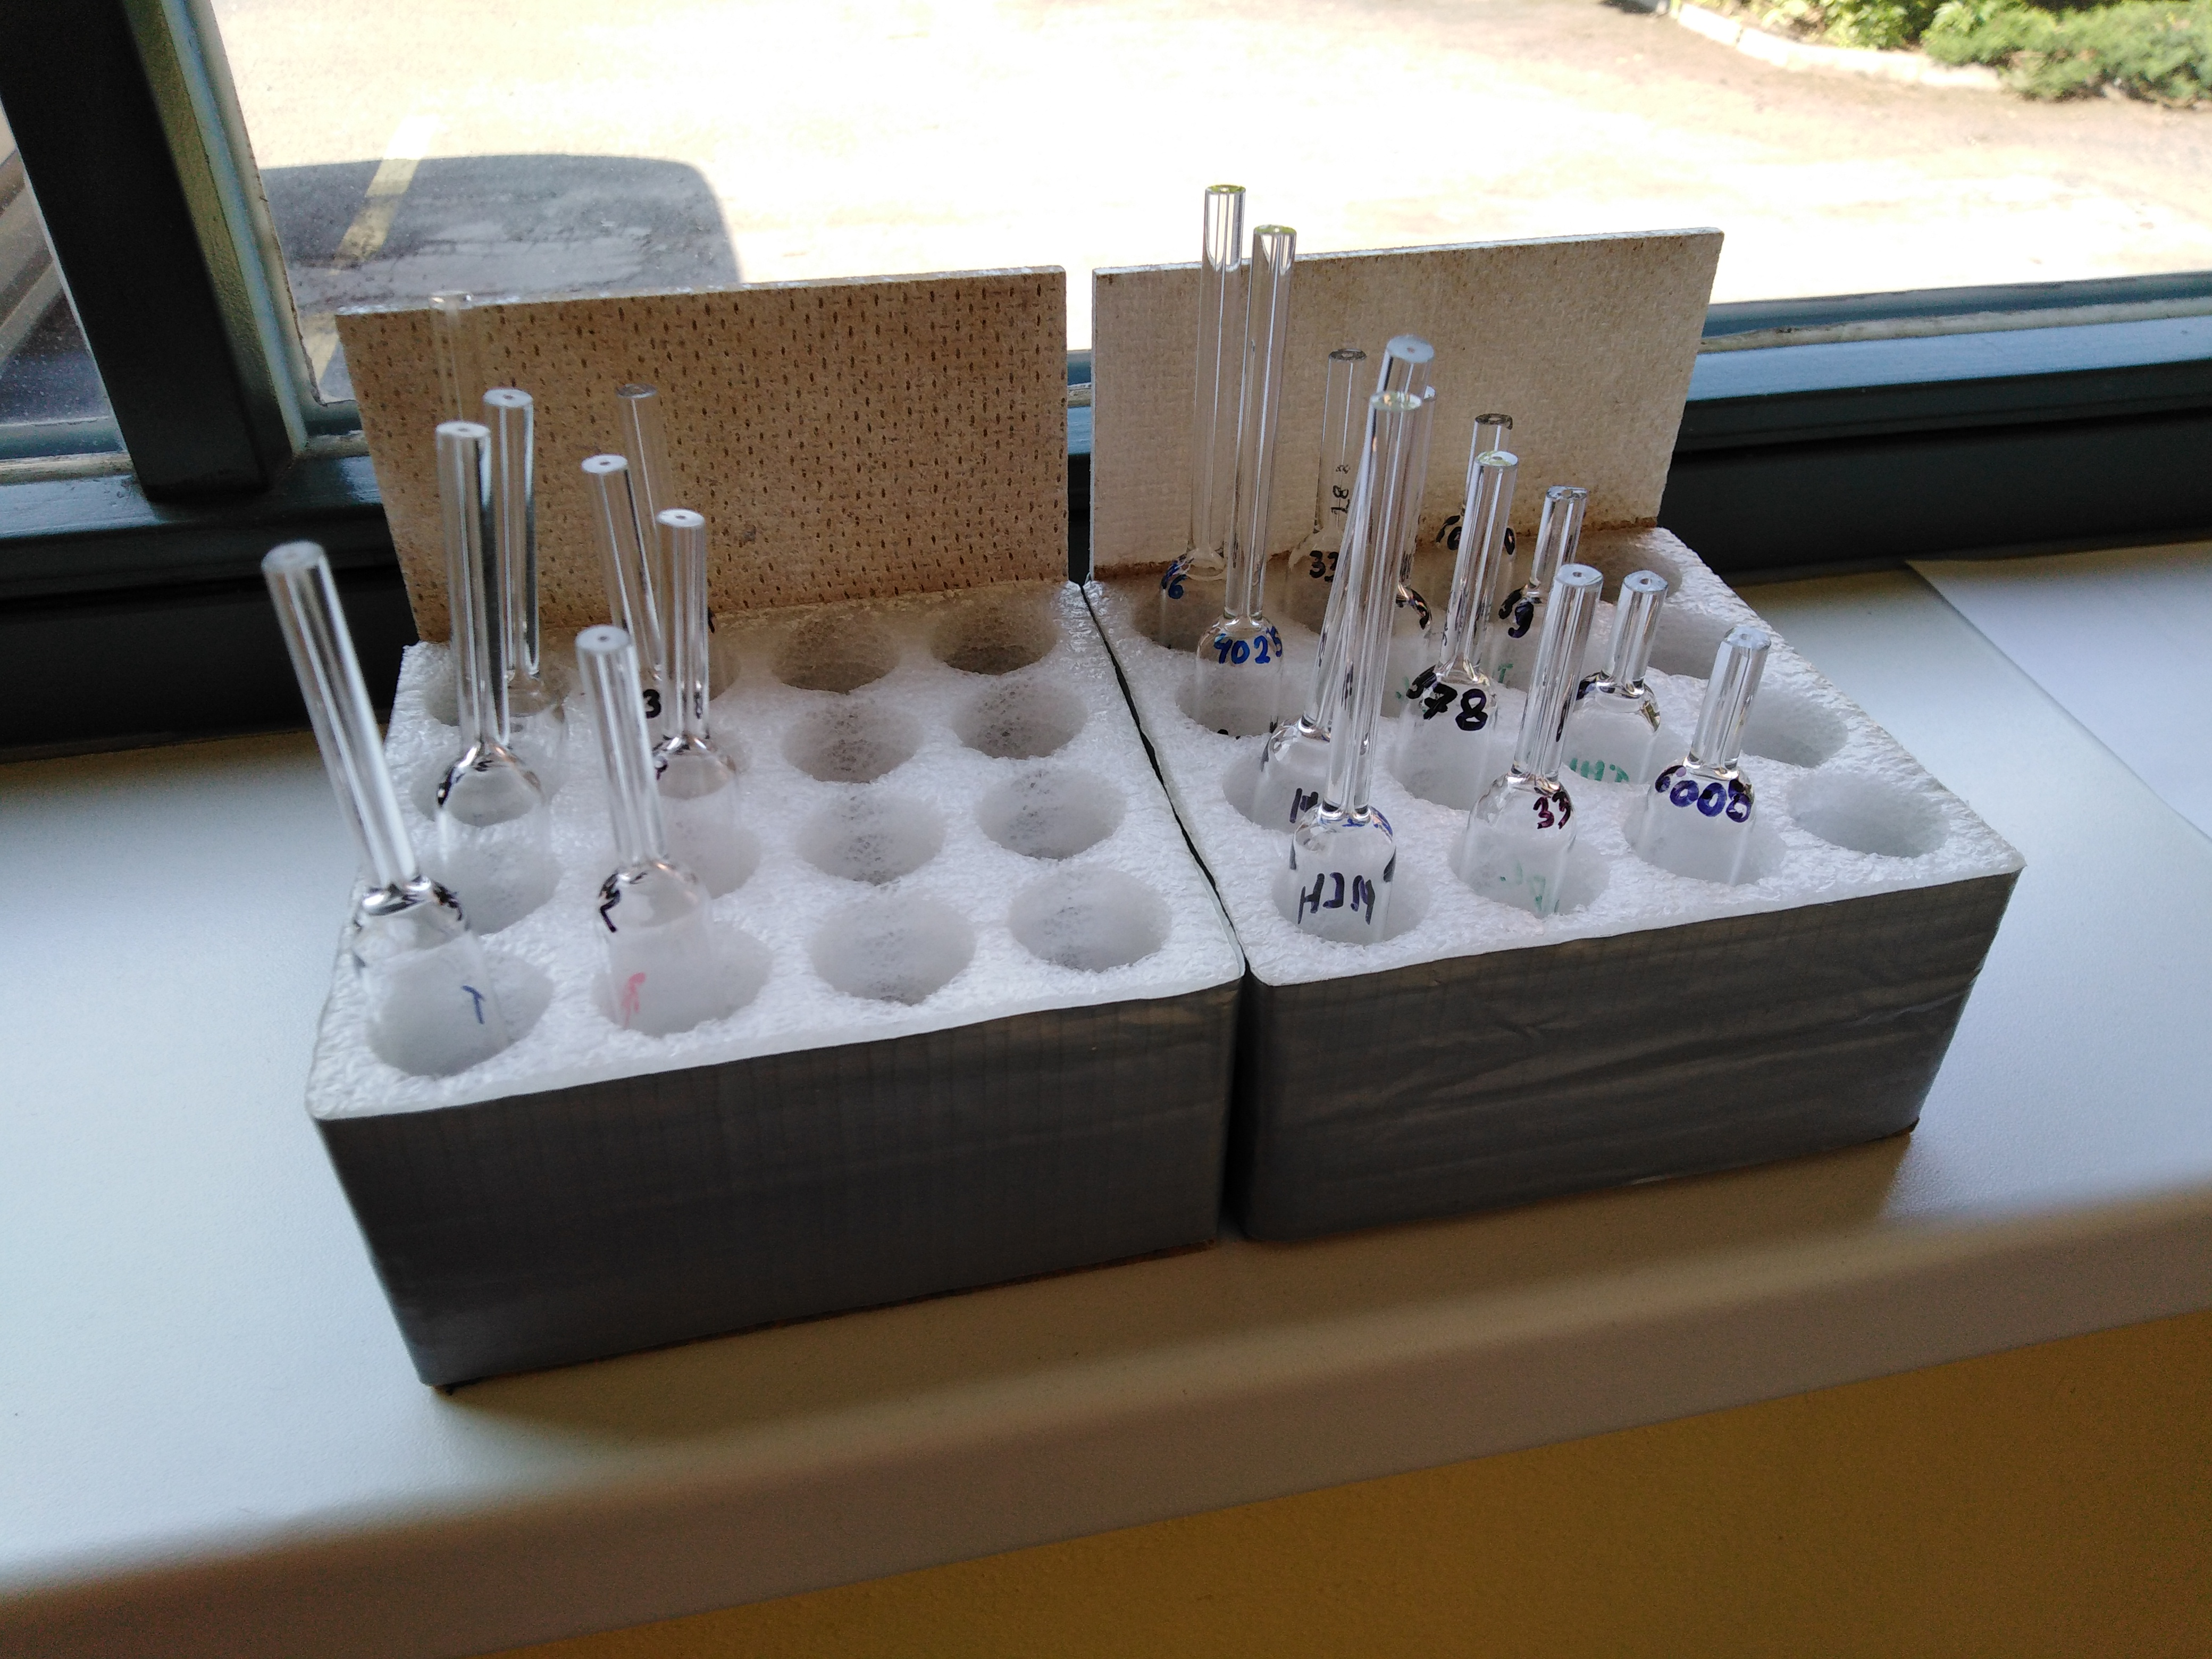
\includegraphics[width=.5\textwidth]{vyvijece_preprava.jpg}
    \caption{Vyvíječe připravené k přepravě.}
    \label{fig:prutoky_vyvijecePreprava}
\end{figure}
\subsection{Instalace měřidel}\label{navesti:prutoky_instalace}
V každé zóně musí být umístěny pouze vyvíječe jednoho typu indikačních plynů, pokud je $N_p=N$. Pokud máme více typů indikačních plynů než je zón, pak mohou být v jedné zóně vyvíječe více typů indikačních plynů, ale vždy musí být v každé zóně zdroj alespoň jednoho typu indikačního plynu, jehož vyvíječe už nejsou v žádné z ostatních zón.

Vyvíječe se umisťují mimo přímé zdroje tepla a chladu. Ideální je umístění 1 až 2 metry od okolních stěn a 0,5 až 1,5 metrů nad zem. Výstup z kapiláry by měl být orientován do středu místnosti. Lze je tedy umisťovat na nábytek, stoly, avšak umístění na parapety oken není vhodné kvůli zvýšenému proudění vzduchu. Nesmíme zapomenout zapsat si časy, kdy byly jednotlivé vyvíječe umístěny.

TD detektory se umisťují vždy alespoň po dvojicích v jednom měřícím místě, přičemž v každé zóně je právě jedno měřící místo. Vzdálenost mezi TD detektory a vyvíječemi by měla minimálně 2 metry a navíc by musí být umístěny na protilehlých stranách místnosti. Dále by měly TD detektory být umístěny ve stejné výšce jako vyvíječe, difúzní uzávěr musí být orientován směrem ke stěně a minimální vzdálenost od stěn by měla být 2~cm. Stejně jako u vyvíječů není doporučeno umisťovat TD detektory na přímé zdroje tepla a chladu a navíc ani do chodeb.

Spolu s vyvíječi by měly být umístěny teploměry testa 174H.

Nesmíme zapomenout zapsat si časy, kdy byly jednotlivá měřidla umístěna.

Více pravidel osazování měřící techniky lze dohledat opět v~\cite{metodika}.

\subsection{Doba měření}
V rámci metodiky~\cite{metodika} jsou uvažována sedmidenní screeningová nebo měsíční integrální měření. Je požadováno stanovení přesnosti doby měření minimálně na jednu hodinu. 

\subsection{Sběr}
Při sběru měřidel si opět zapíšeme časy, kdy byly jednotlivá měřidla sundána ze svých měřících poloh, ideálně s přesností na jednotky minut. Difúzní uzávěry TD detektorů jsou nahrazeny cestovními kovovými. Pravidla přepravy jsou při sběru stejná jako při osazování. Je nutné zaznamenat do formuláře časovou prodlevu mezi sběrem měřidel a jejich předáním k vyhodnocení.

\subsection{Vyhodnocení}
Vyhodnocení TD detektorů se provádí pomocí plynového chromatografu, jehož funkce je popsána výše. Množství odpařeného plynu z vyvíječe se zjišťuje pomocí vážení hmotnosti vyvíječe před a po měření s přesností na desetinu miligramu. Při tom je potřeba vzít do úvahu průběh teploty v zóně, ve které byl vyvíječ umístěn, a také je nutné provést opravu na množství plynu odpařeného v průběhu přepravy.

Vyhodnocování TD detektorů a odparů z vyvíječů je prováděno odbornými pracovníky z oddělení radiochemie SÚRO.

\section{Určení průtoků vzduchu a výměny vzduchu objektu}
Uvažujme nějaký obecný objekt rozdělený na $N$ zón, do něhož byly umístěny vyvíječe $N_p$ indikačních plynů, přičemž musí platit $N_p\geq N$.

\subsection{Hmotnostní koncentrace a emise indikačních plynů}
Z vyhodnocení naměřených dat známe $R_{ki}$, což je průměr odezev TD detektorů umístěných v $i$-té zóně na $k$-tý indikační plyn, průměrnou teplotu $T_i$ a tlak $p_i$ v $i$-té zóně a množství odparu $k$-tého indikačního plynu z vyvíječů umístěných $i$-té zóně. Z tohoto odparu lze určit emisi $k$-tého indikačního plynu v $i$-té zóně:
\begin{equation}
    m_{ki}=\frac{\text{odpar}_{ki}}{dT}\,,
    \label{eq:prutoky_emise}
\end{equation}
kde $dT$ je doba měření ventilace (tj. průtoků a výměny vzduchu) objektu. Z pravidel osazování vyvíječů do kompartmentů plyne $m_{ki}=0$ pro $k\neq i$ (viz oddíl~\ref{navesti:prutoky_instalace}). 

Dále musíme znát molekulové hmotnosti použitých indikačních plynů a odběrové rychlosti TD detektorů všech indikačních plynů.

\begin{table}[ht]
    \centering
    \caption{Molekulové hmotnosti $M$ indikačních plynů a jejich odběrové rychlosti do TD detektorů $U$.~\cite{metodika}}
    \label{tab:prutoky_plyny_konstanty}
    \begin{tabular}{lrr}
        \toprule
ozn. & $M$ [g/mol] & $U$ $\left[\si{\frac{ng}{ppm\cdot min}}\right]$\\
\midrule
TMH & 450,0 &  8,000 \\
TCE & 130,4 &  1,000 \\
MCH & 350,0 &  8,000 \\
MDC & 400,0 &  8,000 \\
PCH & 450,0 &  8,000 \\
PCE & 165,8 &  1,385 \\
\bottomrule
    \end{tabular}
\end{table}

Přehledněji a korektněji jsou tyto veličiny s uvedeny v tab.~\ref{tab:veliciny}, kde jsou uvedeny i jejich jednotky, se kterými se počítá v dalším postupu, pokud není uvedeno jinak.

Následující vztahy jsou přebrány z~\cite{metodika}. Z $R_{ki}, dT, T_i, p_i$ a konstant pro daný indikační plyn $M_k, U_k$ můžeme vypočítat hmotnostní koncentraci $k$-tého indikačního plynu v $i$-té zóně:
\begin{align}
    C_{ki}&=\frac{R_{ki}}{U_k\cdot dT}\frac{M_k}{V_{i}^{mol}}\,,\\
    &=\frac{R_{ki}}{U_k\cdot dT}\frac{M_k\cdot p_i}{R\cdot T_i}\,,
\end{align}
kde bylo využito relace
\begin{equation}
    V^{mol}_{i}=\frac{R\cdot T_i}{p_i}\,.
    \label{eq:prutoky_molarniObjem}
\end{equation}

V tab.~\ref{tab:prutoky_plyny_konstanty} jsou uvedeny molekulové hmotnosti a odběrové rychlosti všech použitých indikačních plynů v rámci tohoto výzkumného úkolu.  
\subsection{Bilanční rovnice}
V rovnovážném stavu se hmotnostní koncentrace indikačních plynů v zónách chovají podle následující soustavy rovnic~\cite{japonci}:
\begin{align}
    \sum_{j=1,j\neq i}^{N}C_{kj}k_{ji}-\sum_{j=1,j\neq i}^{N+1}C_{ki}k_{ij}=-m_{ki}\,,
    \label{eq:prutoky_rovnice}
\end{align}
pro $i\in\{1,2, \ldots, N\}$ a $k\in\{1,2,\ldots, N_p\}$, což nám dává $N\times N_p$ rovnic. Jedná se o bilanční rovnice vyjadřující v podstatě zákon zachování hmotnosti každého z indikačních plynů. V těchto rovnicích vystupují průtoky vzduchu mezi jednotlivými zónami a exfiltrace jednotlivých zón, což jsou veličiny, které chceme určit. Index $N+1$ značí vnější prostředí.

Infiltrace zón lze dopočítat z $N$ průtokových bilančních rovnic \eqref{eq:infiltrace}. Průtokové bilanční rovnice vyjadřují skutečnost, že objem vzduchu jdoucí do dané zóny musí být roven objemu vzduchu vycházejí z této zóny pryč. 

\subsection{Řešení bilančních rovnic}
Pokud máme $N=N_p$, což je nejčastější případ, pak lze soustavu rovnic~\eqref{eq:prutoky_rovnice} řešit analyticky. Uvedeme řešení pro $N=1, 2$:
\begin{itemize}
    \item $N=1$
        \begin{equation}
            k_E=\frac{m}{C}\,.
        \end{equation}
    \item $N=2$
        \begin{align}
            k_{21}&=\frac{m_{11}C_{21}}{C_{11}C_{22}-C_{12}C_{21}}\,, \\
            k_{12}&=\frac{m_{22}C_{12}}{C_{11}C_{22}-C_{12}C_{21}}\,, \\
            k_{1_E}&=k_{21}\frac{C_{22}}{C_{21}}-k_{12}\,,\\
            k_{2_E}&=k_{12}\frac{C_{11}}{C_{12}}-k_{21}\,.
        \end{align}
\end{itemize}
Pro vyšší $N$ nabývá řešení rychle na složitosti. Pro zjednodušení jsem napsal v Pythonu skript využívající symbolického programování pro vyřešení soustavy pro obecné $N$. Naneštěstí je velmi pomalý, pro $N=3$ trvá výpočet přibližně 18 vteřin a pro $N=4$ jsem výpočet přerušil, protože trval příliš dlouho.

K propagaci nejistot od vstupních veličin k průtokům vzduchu jsem využil pythonovský balíček~\cite{uncertainties}.
\subsubsection{Lineární regrese}
Obecnější řešení nabízí lineární regrese, kterou lze použít i pro přeurčenou soustavu rovnic, kterou dostáváme při $N_p>N$. Aby jí šlo využít, tak je potřeba přepsat soustavu~\eqref{eq:prutoky_rovnice} do tvaru 
\begin{equation}
    X\beta=y\,,
    \label{eq:prutoky_regrese}
\end{equation}
kde $\beta$ je vektor parametrů k určení o $N^2$ složkách, $X$ je matice o rozměrech $(N\cdot N_p)\times N^2$ a $y$ je vektor o $N\cdot N_p$ složkách:
\begin{align}
    \beta=
    \begin{pmatrix}
        k_{12}\\
        k_{13}\\
        \vdots\\
        k_{1,N+1}\\
        k_{21}\\
        k_{23}\\
        \vdots\\
        k_{2,N+1}\\
        \vdots\\
        k_{N,N-1}\\
        k_{N,N+1}
    \end{pmatrix}\,,\qquad y=
    -\begin{pmatrix}
        m_{11}\\
        m_{12}\\
        \vdots\\
        m_{1,N+1}\\
        m_{21}\\
        m_{22}\\
        \vdots\\
        m_{2,N+1}\\
        \vdots\\
        m_{N,N}\\
    \end{pmatrix}=
    \begin{pmatrix}
        -m_{11}\\
        0\\
        \vdots\\
        0\\
        0\\
        -m_{22}\\
        \vdots\\
        0\\
        \vdots\\
        -m_{N,N}\\
    \end{pmatrix}
    \,.
\end{align}
Nulovost $m_{ki}$ pro $k\neq i$ plyne z pravidel pro osazování vyvíječů do zón. Matice $X$ je určena následovně: pokud je $m$-tá složka vektoru $\beta$ průtok $k_{ij}$, pak 
\begin{align}
    X_{N_p\cdot k-N_p+i,m}&=-C_{ki}\,,\\
    X_{N_p\cdot k-N_p+j,m}&=C_{ki}\,.
\end{align}
Pokud řádkový index ($N_p\cdot k-N_p+i$, resp. $N_p\cdot k-N_p+j$) přesáhne řádkový rozměr matice $X$, pak je ignorován a žádná hodnota se nikam nepřiřazuje. Pro vysvětlení uvažujme $k=1$. Pak výše uvedené vztahy říkají, že prvek matice $X$ v $i$-tém řádku a $m$-tém sloupci je roven $-C_{1i}$ a prvek v $j$-tém řádku a $m$-tém sloupci $C_{1i}$. Výraz $N_p\cdot k-N_p$ je potřeba pro dopočet ostatních prvků matice, které jsou odvozeny od koncentrací ostatních indikačních plynů. Při odvozování matice $X$ jsem postupoval podle článku~\cite{japonci2}.

Nevýhodou této metody je, že nedokáže určit nejistoty vypočtených průtoků vzduchu při $N=N_{p}$. 

Tento postup výpočtu jsem také implementoval v Pythonu a pro $N=N_{p}$ vychází analytické a regresní řešení stejně, výhodou analytického řešení je určení nejistot řešení. 

Skripty analytického ani regresního řešení v této práci neuvádím, jelikož využívají podobných principů jako skripty určené pro výpočet přísunů radonu do zón (viz další kapitola).

\subsection{Výměna vzduchu}
Pokud známe exfiltrace a objemy všech zón, pak můžeme vypočítat výměnu vzduchu objektu:
\begin{equation}
    n=\frac{\sum_{i=1}^N k_{i_E}}{\sum_{i=1}^N V_i}\,.
    \label{eq:prutoky_n}
\end{equation}
Udává se v \si{1/hod} a vyjadřuje podíl objemu vzduchu, který za jednu hodinu unikne z objektu do vnějšího prostředí, a celkového objemu vzduchu uvnitř objektu (tj. vlastně součtu objemů všech zón).
